% ----------------------------------------------------------------------------
% Section 6.8 --- Black Hole Evaporation and the Information Problem
% From former §7.8, heavily condensed
% ----------------------------------------------------------------------------
\subsection{Black Hole Evaporation and the Information Problem}
\label{subsec:black-hole-evaporation-information}

Black hole evaporation is an effective process arising from the gradual
restoration of projectability near the boundary separating projectable and
non-projectable domains.
The apparent information loss identified by
Hawking~\cite{Hawking1976} arises from applying a spacetime-based
description beyond its domain of validity.
In Cosmochrony, information is encoded in the global relational
configuration independently of its spacetime projection.

\subsubsection*{Horizon Reprojection Equation}
\label{subsec:horizon-reprojection-equation}

The energy flux emerging from the horizon is a sum over discrete
reprojection events:
\[
  \Phi_\chi \equiv \frac{dE}{dt}
  = \sum_k \delta(t - t_k)\,
    \hbar_\chi\, \nu_k(L_{\mathrm{sol}}).
\]
Here $\hbar_\chi$ is the fundamental quantum of reprojection, the
$\nu_k(L_{\mathrm{sol}})$ are resonance frequencies of the stability
operator at the horizon, and $t_k$ label the instants at which local
configurations reach the projection threshold.

\subsubsection*{Emergent Temperature and Relaxation Gradient}
\label{subsec:emergent-temperature}

The apparent Hawking temperature is determined by the gradient of
effective $\chi$ relaxation normal to the horizon:
\[
  k_B T_\chi = \frac{\hbar_\chi c}{2\pi}\,
  \left| \nabla_{\perp} \chi_{\mathrm{eff}}
  \right|_H.
\]
For more massive black holes, the relaxation gradient is distributed over
a larger area, reducing the frequency of reprojection events and
explaining the inverse mass--temperature relation without invoking vacuum
particle creation.

\subsubsection*{Information Conservation and Spectral Encoding}
\label{subsec:information-conservation}

During deprojection, information is stored in the nonlinear degrees of
freedom of~$\chi$ within the projection fiber.
During reprojection, each emitted quantum carries the spectral imprint of
the eigenmodes governing the $\chi$ configuration, ensuring global
information conservation.

\subsubsection*{Entropy as a Projection Saturation Limit}
\label{subsubsec:entropy-projection-saturation}

The Bekenstein--Hawking area law
\begin{equation}
  S = \frac{A}{4}
\end{equation}
is reinterpreted as the informational capacity of the projection map at
the horizon boundary.
Entropy quantifies hidden relational structure---the structural
multiplicity of $\chi$ configurations no longer distinguishable at the
metric level---rather than thermal ignorance.

\begin{figure}[htbp]
  \centering
  \resizebox{\linewidth}{!}{%
    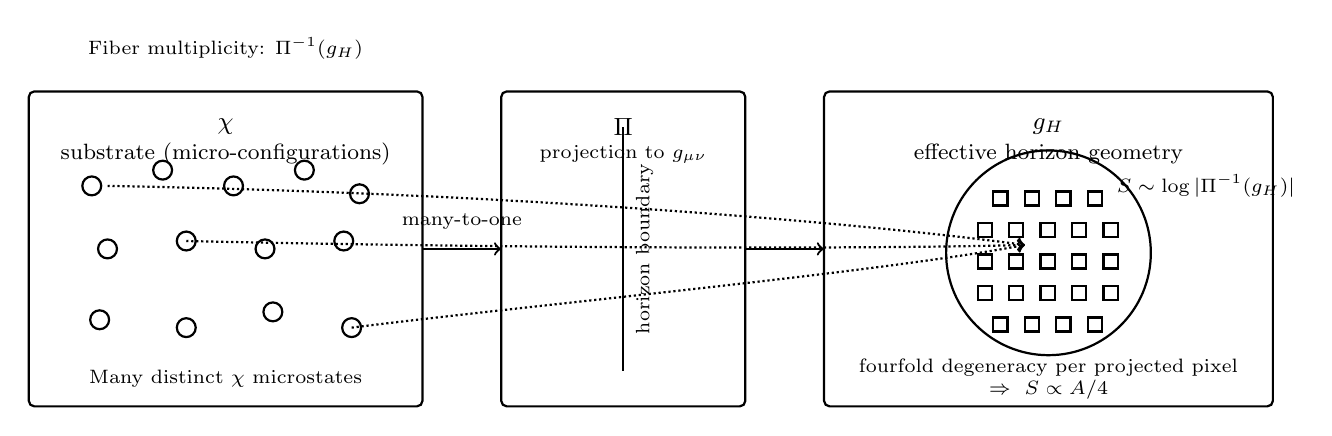
\begin{tikzpicture}[font=\small]
      \draw[thick,rounded corners=2pt] (0,0) rectangle (5.0,4.0);
      \node at (2.5,3.55) {$\chi$};
      \node[font=\footnotesize] at (2.5,3.20)
        {substrate (micro-configurations)};
      \draw[thick,rounded corners=2pt] (6.0,0) rectangle (9.1,4.0);
      \node at (7.55,3.55) {$\Pi$};
      \node[font=\scriptsize] at (7.55,3.20)
        {projection to $g_{\mu\nu}$};
      \draw[thick,rounded corners=2pt]
        (10.1,0) rectangle (15.8,4.0);
      \node at (12.95,3.55) {$g_H$};
      \node[font=\footnotesize] at (12.95,3.20)
        {effective horizon geometry};
      \foreach \x/\y in {0.8/2.8,1.7/3.0,2.6/2.8,3.5/3.0,
        4.2/2.7,1.0/2.0,2.0/2.1,3.0/2.0,4.0/2.1,
        0.9/1.1,2.0/1.0,3.1/1.2,4.1/1.0}{
        \draw[thick] (\x,\y) circle (0.12);
      }
      \node[font=\scriptsize] at (2.5,0.35)
        {Many distinct $\chi$ microstates};
      \draw[->,thick] (5.0,2.0) -- (6.0,2.0);
      \node[font=\scriptsize] at (5.5,2.35) {many-to-one};
      \draw[thick] (7.55,0.45) -- (7.55,3.55);
      \node[font=\scriptsize,rotate=90] at (7.82,2.0)
        {horizon boundary};
      \draw[->,thick] (9.1,2.0) -- (10.1,2.0);
      \draw[thick] (12.95,1.95) circle (1.30);
      \foreach \x/\y in {12.25/2.55,12.65/2.55,
        13.05/2.55,13.45/2.55,
        12.05/2.15,12.45/2.15,12.85/2.15,
        13.25/2.15,13.65/2.15,
        12.05/1.75,12.45/1.75,12.85/1.75,
        13.25/1.75,13.65/1.75,
        12.05/1.35,12.45/1.35,12.85/1.35,
        13.25/1.35,13.65/1.35,
        12.25/0.95,12.65/0.95,
        13.05/0.95,13.45/0.95}{
        \draw[thick] (\x,\y) rectangle ++(0.18,0.18);
      }
      \draw[->,thick,densely dotted] (1.0,2.8)
        .. controls (6.5,2.7) and (10.8,2.3)
        .. (12.65,2.05);
      \draw[->,thick,densely dotted] (2.0,2.1)
        .. controls (6.5,2.0) and (10.8,2.0)
        .. (12.65,2.05);
      \draw[->,thick,densely dotted] (4.1,1.0)
        .. controls (6.5,1.3) and (10.8,1.7)
        .. (12.65,2.05);
      \node[font=\scriptsize,align=left] at (2.5,4.55)
        {Fiber multiplicity: $\Pi^{-1}(g_H)$};
      \node[font=\scriptsize,align=left] at (14.95,2.80)
        {$S \sim \log |\Pi^{-1}(g_H)|$};
      \node[font=\scriptsize,align=center] at (12.95,0.35)
        {fourfold degeneracy per projected pixel\\
         $\Rightarrow\ S \propto A/4$};
    \end{tikzpicture}%
  }
  \caption{Saturation of the projection map at the horizon.
    Multiple micro-configurations of~$\chi$ collapse onto the same
    effective horizon geometry~$g_H$.
    Entropy measures the structural multiplicity of the fiber
    $\Pi^{-1}(g_H)$.}
  \label{fig:projection-saturation-horizon}
\end{figure}

\subsubsection*{Prediction: Spectral Granularity}
\label{subsec:spectral-granularity}

If Hawking radiation is fundamentally discrete, it cannot be a perfect
black-body continuum.
The spectral line width of a reprojected quantum is
\begin{equation}
  \Delta \nu_k \approx
    \frac{1}{\tau_\chi}\, \sqrt{\alpha}\, \ln(Q),
\end{equation}
where $\tau_\chi$ is the characteristic relaxation time near the horizon,
$\alpha \simeq 3 \times 10^{-7}$ is the spectral packing fraction, and
$Q$ is the topological charge of the emitted configuration.
The ratio between line width and line spacing is universally governed
by~$\alpha$:
\begin{equation}
  \frac{\Delta \nu}{\delta \nu} \propto \alpha .
\end{equation}

\subsubsection*{Observational Prospects}
\label{subsec:observational-granularity}

In the late stages of evaporation, the spectral spacing may enter the
sensitivity bands of next-generation interferometers (LISA, Einstein
Telescope).
The universal relation $\Delta \nu / \delta \nu \simeq \alpha$ should
also apply to analogue gravity systems, where current experiments in
Bose--Einstein condensates approach the required spectral resolution
($\delta f / f \sim 10^{-5}$), making near-term tests feasible.
